\chapter{STM32H745 Microcontroller}

The STM32H745 is a heterogeneous dual-core microcontroller from STMicroelectronics. For this task I was able to acquire a Nucleo-H745 development board which has a number of useful peripherals besides the aforementioned MCU chip.

\section{Choosing the right hardware}

In the early stages of the project 2 microcontrollers were offered for the task. A quad-core MCU from Texas Instruments with homogeneous architecture and the STM32H745.

After taking a glance at the then current state of multicore Rust, it seemed that a homogeneous device would be the better choice. However the TI MCU was not on a good development board in the sense that it did not have many peripherals which would be required in the second part of the project, as making some external hardware would not fit in the time frame. Besides this, Texas Instruments microcontrollers are yet to receive rust support. Implementing all the necessary drivers in Rust for a new MCU is certainly possible, but a task like that alone could fill the whole project and is not in the area of study this thesis aims to explore.

The other candidate, the STM32H745 had only one small drawback it being a heterogeneous architecture. In all other aspects it was the better choice for this project. STM32 microcontrollers have considerable Rust support regarding peripheral drivers that implement the HAL (Hardware Abstraction Layer). On top of this, some development boards also have BSP-s (Board Support Package) that implement another abstraction layer above the HAL by hiding even the pin numbers. For example, to turn on a LED with a HAL crate, the user would need to set the \mycode{PB0} pin, but with a BSP one could call a function similar to \mycode{SetLed(1)} and achieve the same effect without looking up the pin that corresponds to the LED. In other words the HAL is for the MCU, while the BSP is for the whole development board. An incomplete BSP exists for the Nucleo-H745 but for reasons explained later, this project will only include the HAL crate for the MCU.

\begin{figure}[!ht]
    \centering
    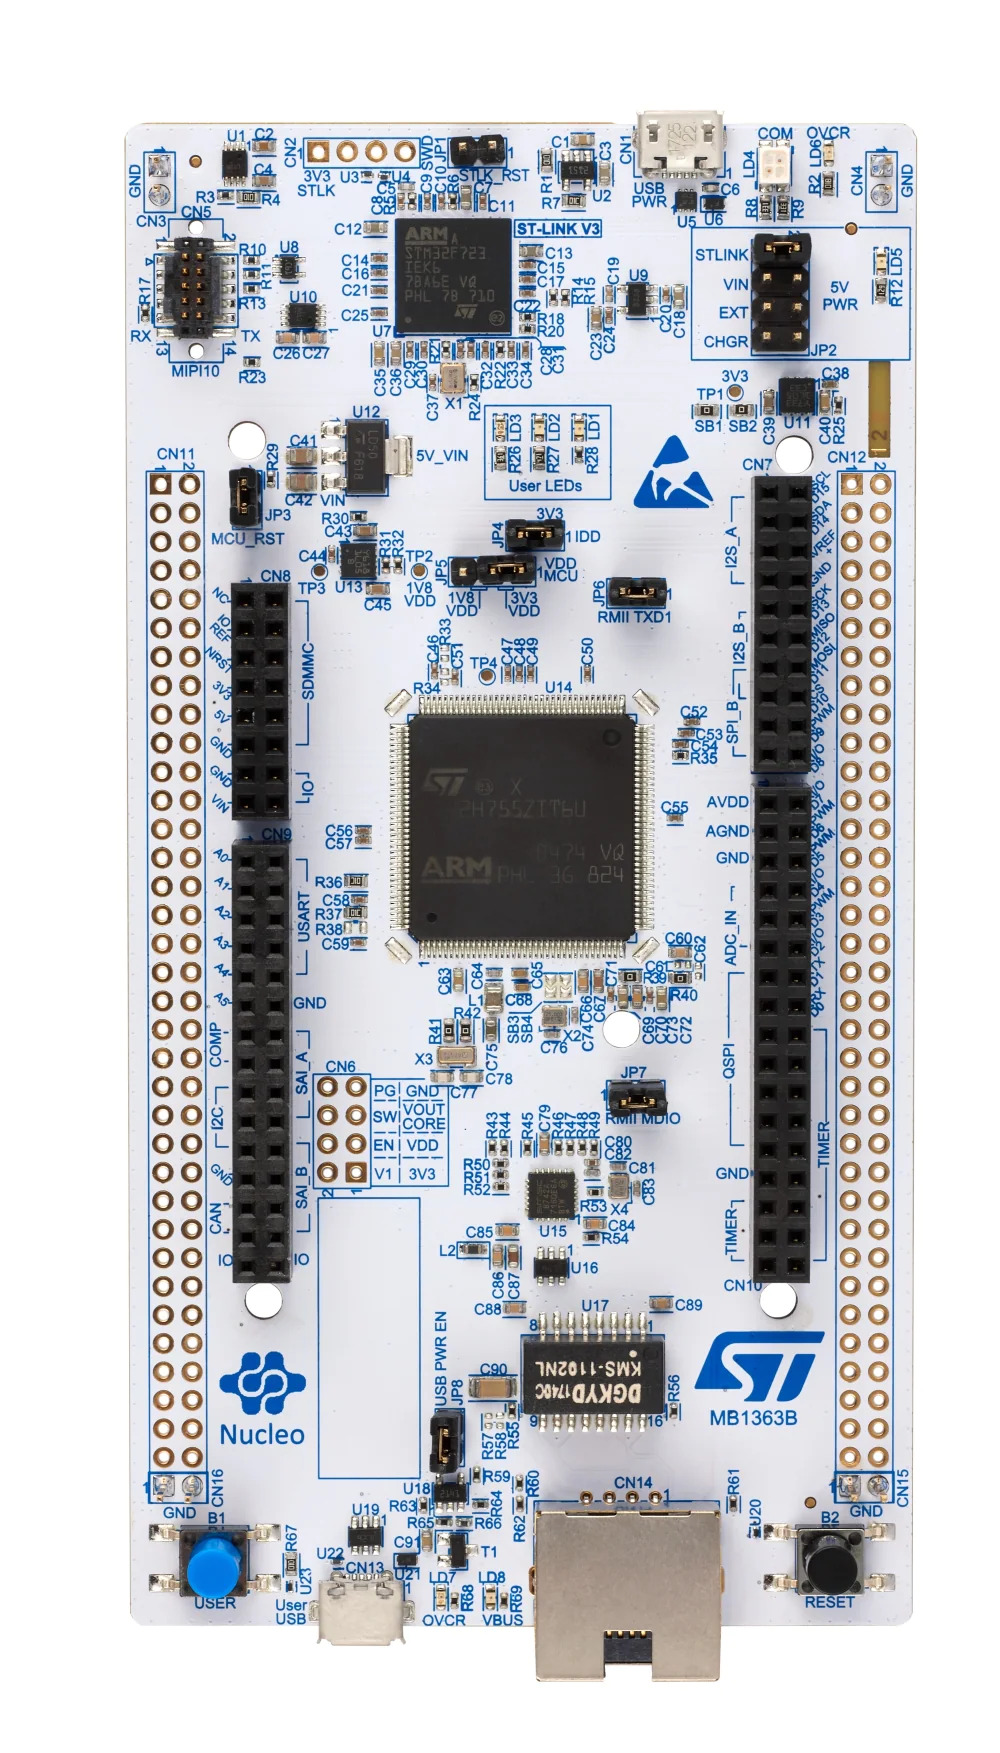
\includegraphics[height=150mm, keepaspectratio, angle=90]{figures/devboard.jpg}
    \caption{The STM32 Nucleo-H745 Development Board}
    \label{fig:Nucleo-H745}
\end{figure}

\section{Hardware Capabilities}

\subsection{Power}

Power can be provided to the MCU in a variety of ways and with different voltages ranging from 3.3 to 11 Volts. This makes it easy for developers to integrate this microcontroller into their designs. In this project however, only the development board will be used. The easiest way to power the development board is through a microUSB port, which is also used for programming and debugging. As connection to a PC is already needed in this early stage of development, the fact that power is also derived from this connection makes this setup comfortable to use or move.

\subsection{Clocks}

In the default setup the MCU starts with an external clock signal that originates from the Board Management Controller. This controller is also responsible for programming and debugging. The microcontroller contains internal oscillators as well as PLL-s. The usage of these can be configured in runtime during the setup phase of an application. Usually in the first part of initializing the application the clock is set, in this case a PLL will be used with the external clock signal from the Board Controller used as reference.

There are several clock domains which makes it possible to fine tune our application for low power consumption. Configuration code can be generated using official tools from the manufacturer using a GUI application. A maximum frequency of 240 MHz can be achieved for the M7 core and 120 MHz for the M4 core.

\subsection{Analog interfaces}

\subsubsection{Analog Digital Converter}

Almost all modern microcontrollers include some kind of analog to digital converter peripheral and the STM32H745 is not an exception. \cite{ADCDescription} It has three ADC-s where ADC1 and ADC2 are tightly coupled with ADC1 being the master while ADC3 is fully independent. Each ADC consists of a 16-bit successive approximation analog-to-digital converter and has up to 20 multiplexed channels. A/D conversion of the various channels can be performed in single, continuous, scan or discontinuous mode. The result of the conversion is stored in a left-aligned or right-aligned 32-bit data register.

The ADC-s can use a lower resolution than 16 bit to decrease conversion time which is also independent of the AHB bus clock frequency. The ADC-s are capable of self calibration which reduces the complexity of their initialization. The start of a conversion can be initiated either by means of the software calling the applicable driver function, or hardware triggers, ie. interrupts of timer events. They are also capable of sending in interrupt themselves when a conversion is finished.

There are two main modes of using an ADC. The easiest method is using single conversion mode. With this mode, all the channel conversions are started and once these are finished, the results are stored in the appropriate registers and an end of conversion flag is checked. This way a blocking call to an ADC conversion can be easily implemented by waiting for the end of conversion flag to be flipped. The second way is continuous conversion mode. Here, instead of stopping after the conversion is done and the result is placed in a register, the ADC will start this process again. When a conversion is finished it sends an interrupt that the data should be extracted from the register. Not handling this interrupt properly (ie. not saving the content of this register) will not stop the ADC from overwriting the content of the register.

The timing of a conversion can be useful information when designing an application. The elapsed time between the start of a conversion and the end of conversion is the sum of the configured sampling time plus the successive approximation time depending on data resolution can be calculated according to the following formula.

\[T_{CONV} = T_{SMPL} + T_{SAR} = [1.5_{|min} + 7.5_{|14bit}] \times T_{adc\_ker\_ck}\]

\[ T_{CONV} = 62.5 ns_{|min} + 312.5 ns_{|14bit} = 375.0 ns\]

Where $T_{SMPL}$ is the sampling time which depends on the channel and $T_{SAR}$ depends in the resolution. In the formula above $T_{adc\_ker\_ck}$ equals 24 MHz, the resolution is 14 bit, and the lowest possible sampling time is substituted to demonstrate its usage.

\begin{figure}[!ht]
    \centering
    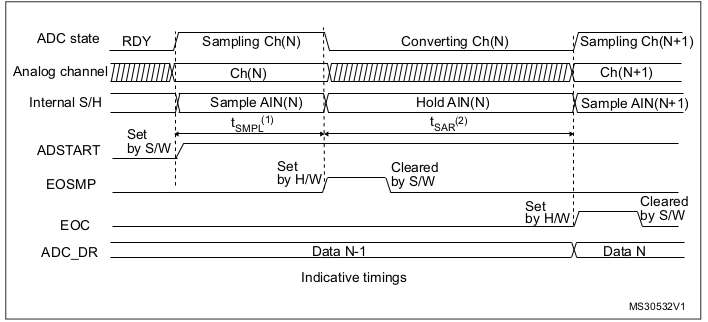
\includegraphics[width=150mm, keepaspectratio]{figures/adc-timing.png}
    \caption{Analog to Digital Conversion Time\cite{ADConversionTime}}
    \label{fig:adc-timing}
\end{figure}

\subsubsection{Digital Analog Converter}

\subsection{Connectivity}

\subsubsection{Programming and debugging}

This development board is equipped with an on-board ST-LINK debugger and programmer. This module can handle the USB connection to a computer and also act a virtual COM port or a debug port. There are multiple ways of programming the device using the ST-LINK connection, a programmer is available in the official STM IDE (Integrated Development Environment) but there are also standalone command line and GUI tools for programming. Any suitable debugger can connect to the debug port of the ST-LINK module, debugging will be described more in-depth in a further chapter.

\subsubsection{Ethernet}

Both cores of the microcontroller have pins that can be considered to use an ethernet interface. The development board has an ethernet connector that is compliant with the IEE-802.3-2002 standard. The ethernet connector is a really interesting feature for this project as in the second part when developing a more complex application. Such an application would be able to provide a minimal webGUI (Graphical User Interface) thanks to the ethernet connector.

\subsubsection{USB}

The development board has in total 2 USB Micro-AB connectors. One of them is connected to the previously mentioned ST-LINK connector so it cannot be configured freely. However the other one is fully available for the programmer to use. Most likely this project will not utilize the USB port, but with similar complexity, and sometimes similar speeds, it could replace the ethernet port as another high-speed communication interface if needed.

\subsubsection{USART}

There are multiple pins that can be configured for USART peripherals, however the most important in this case is the one available through the \mycode{PD8} and \mycode{PD9} pins, which can be connected to the ST-LINK connector. By doing this we have a way of communicating with our program through a trivial communication protocol that requires minimal setup and driver support, and using the same USB port we used for powering and programming the board. Throughout development this port will be used for displaying debug traces.

\subsection{Other useful peripherals}

\subsubsection{GPIO-s}

As the pins of the STM32H745 MCU are very configurable and 144 pins are routed onto the development board, there is a considerable amount of GPIO-s that can be utilized if needed, though many of them are taken by other peripherals on the board. Three GPIO-s are each routed to a different colored user LED on the board, which is extremely useful in early bring-up of a board as blinking an LED is often considered the "Hello World of hardware related projects". Also present on the board are 2 buttons, one of which is a dedicated reset button while the other can be configured by the user.

\subsubsection{Hardware semaphores}

The hardware semaphore block on this system provides 32 32-bit register based semaphores. The semaphores can be used to ensure synchronization between different processes running between different cores. They provide a non-blocking mechanism to lock semaphores in an atomic way even when multiple cores are trying to access them at the same time. There are two ways of locking one of these hardware semaphores. The first method is useful when not only the other core, but some other process from any core could try to access the semaphore. With this method, the \mycode{COREID} and \mycode{PROCID} are written to the semaphore, followed by a read check. A one-step-lock is also available, where only the \mycode{COREID} is read from the semaphore.

The semaphores are able to generate an interrupt on any of the interrupt lines, this needs to be configured during peripheral initialization phase. A semaphore is only cleared when \mycode{COREID} and \mycode{PROCID} match, except that a global clear is available per \mycode{COREID}. All 32 hardware semaphores have the following features: 8-bit PROCID, 4-bit COREID, 2 interrupt lines, and lock indication.

The semaphore is free when its LOCK bit is 0. In this case, the COREID and PROCID are also 0. When the LOCK bit is 1, the semaphore is locked and the COREID indicates which AHB bus master locked it. The PROCID indicates which process of that AHB (Advanced High-performance Bus) bus master locked the semaphore. When write locking a semaphore, the COREID is taken from the master ID and the PROCID is taken from the write data. When read locking the semaphore, the COREID is taken from the AHB bus master ID, and the PROCID is zero. There is no PROCID available with the 1- step (read) lock. The COREID is taken from the AHB bus master ID. The PROCID is written by the software of that AHB bus master. Each AHB bus master process must have a unique PROCID. PROCID is only available in the 2-step lock procedure.

\begin{figure}[!ht]
    \centering
    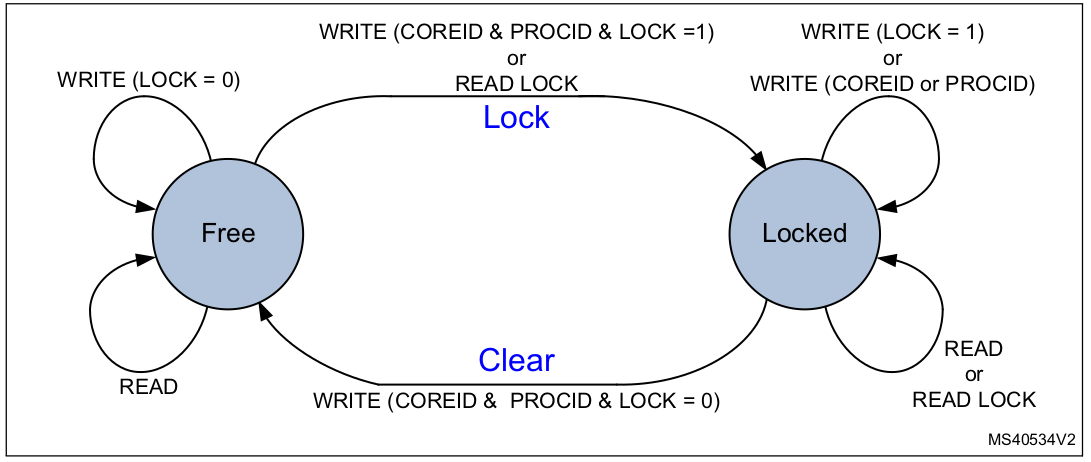
\includegraphics[width=150mm, keepaspectratio]{figures/hw-semaphore.png}
    \caption{Hardware semaphore state diagram \cite{HWSemaphore}}
    \label{fig:HWSemaphore}
\end{figure}

Clearing a semaphore is a protected process, to prevent accidental clearing by a AHB bus master or by a process that does not have the semaphore lock right. The semaphore clear procedure consists in writing to the semaphore with the corresponding COREID and PROCID and LOCK = 0. When cleared, the semaphore LOCK, the COREID, and the PROCID are all 0. When cleared, an interrupt may be generated to signal the event. To this end, the semaphore interrupt must be enabled.
